\documentclass[10pt]{beamer}
\usepackage{amsmath}
\usepackage{mathtools}
\usepackage{multimedia}
\usepackage{hyperref}


\usefonttheme{professionalfonts} % using non standard fonts for beamer
\usefonttheme{serif} % default family is serif
%\documentclass[12pt]{beamerthemeSam.sty}
\usepackage{epsf}
%\usepackage{pstricks}
%\usepackage[orientation=portrait,size=A4]{beamerposter}
\geometry{paperwidth=160mm,paperheight=120mm}
%DT favorite definitions
\def\LL{\left\langle}	% left angle bracket
\def\RR{\right\rangle}	% right angle bracket
\def\LP{\left(}		% left parenthesis
\def\RP{\right)}	% right parenthesis
\def\LB{\left\{}	% left curly bracket
\def\RB{\right\}}	% right curly bracket
\def\PAR#1#2{ {{\partial #1}\over{\partial #2}} }
\def\PARTWO#1#2{ {{\partial^2 #1}\over{\partial #2}^2} }
\def\PARTWOMIX#1#2#3{ {{\partial^2 #1}\over{\partial #2 \partial #3}} }

\def\rightpartial{{\overrightarrow\partial}}
\def\leftpartial{{\overleftarrow\partial}}
\def\diffpartial{\buildrel\leftrightarrow\over\partial}

\def\BC{\begin{center}}
\def\EC{\end{center}}
\def\BN{\begin{enumerate}}
\def\EN{\end{enumerate}}
\def\BI{\begin{itemize}}
\def\EI{\end{itemize}}
\def\BE{\begin{displaymath}}
\def\EE{\end{displaymath}}
\def\BEA{\begin{eqnarray*}}
\def\EEA{\end{eqnarray*}}
\def\BNEA{\begin{eqnarray}}
\def\ENEA{\end{eqnarray}}
\def\EL{\nonumber\\}

\newcommand{\etal}{{\it et al.}}
\newcommand{\gbeta}{6/g^2}
\newcommand{\la}[1]{\label{#1}}
\newcommand{\ie}{{\em i.e.\ }}
\newcommand{\eg}{{\em e.\,g.\ }}
\newcommand{\cf}{cf.\ }
\newcommand{\etc}{etc.\ }
\newcommand{\atantwo}{{\rm atan2}}
\newcommand{\Tr}{{\rm Tr}}
\newcommand{\dt}{\Delta t}
\newcommand{\op}{{\cal O}}
\newcommand{\msbar}{{\overline{\rm MS}}}
\def\chpt{\raise0.4ex\hbox{$\chi$}PT}
\def\schpt{S\raise0.4ex\hbox{$\chi$}PT}
\def\MeV{{\rm Me\!V}}
\def\GeV{{\rm Ge\!V}}

%AB: my color definitions
%\definecolor{mygarnet}{rgb}{0.445,0.184,0.215}
%\definecolor{mygold}{rgb}{0.848,0.848,0.098}
%\definecolor{myg2g}{rgb}{0.647,0.316,0.157}
\definecolor{A}{rgb}{1.0,0.3,0.3}
\definecolor{B}{rgb}{0.0,1.0,0.0}
\definecolor{C}{rgb}{1.0,1.0,0.0}
\definecolor{D}{rgb}{0.5,0.5,1.0}
\definecolor{E}{rgb}{0.7,0.7,0.7}
\definecolor{abtitlecolor}{rgb}{1.0,1.0,1.0}
\definecolor{absecondarycolor}{rgb}{0.0,0.416,0.804}
\definecolor{abprimarycolor}{rgb}{1.0,0.686,0.0}
\definecolor{Red}           {rgb}{1,0.4,0.4}
\definecolor{Yellow}           {rgb}{1,1,0.0}
\definecolor{Grey}          {cmyk}{.7,.7,.7,0}
\definecolor{Blue}          {cmyk}{1,1,0,0}
\definecolor{Green}         {cmyk}{1,0,1,0}
\definecolor{Brown}         {cmyk}{0,0.81,1,0.60}
\definecolor{Silver}        {rgb}{0.95,0.9,1.0}
\definecolor{Sky}           {rgb}{0.07,0.0,0.2}
\definecolor{Darkbrown}     {rgb}{0.4,0.3,0.2}
\definecolor{40Gray}        {rgb}{0.4,0.4,0.5}
\usetheme{Madrid}


\setbeamercolor{normal text}{fg=Silver,bg=Sky}

%AB: redefinition of beamer colors
%\setbeamercolor{palette tertiary}{fg=white,bg=mygarnet}
%\setbeamercolor{palette secondary}{fg=white,bg=myg2g}
%\setbeamercolor{palette primary}{fg=black,bg=mygold}
\setbeamercolor{title}{fg=abtitlecolor}
\setbeamercolor{frametitle}{fg=abtitlecolor}
\setbeamercolor{palette tertiary}{fg=white,bg=Darkbrown}
\setbeamercolor{palette secondary}{fg=white,bg=absecondarycolor}
\setbeamercolor{palette primary}{fg=white,bg=40Gray}
\setbeamercolor{structure}{fg=abtitlecolor}

\setbeamerfont{section in toc}{series=\bfseries}

%AB: remove navigation icons
\beamertemplatenavigationsymbolsempty
\title[The yearly motion of the sky]{
  \textbf {The yearly motion of the sky}
}

\author [Astronomy 101]{Astronomy 101\\Syracuse University, Fall 2016\\Walter Freeman}

\date{\today}

\begin{document}



\frame{\titlepage}


\frame{\frametitle{\textbf{The Sun and the stars: the zodiac}}
\large
This is the excellent foppery of the world, that, when we are
sick in fortune, often the surfeit of our own behaviour, we make
guilty of our disasters the sun, the moon, and the stars; as if
we were villains on necessity; fools by heavenly compulsion... 
An admirable evasion of whore-master man, to lay
his goatish disposition to the charge of a star!

\bigskip
\bigskip

\begin{flushright}---William Shakespeare, {\it King Lear}\end{flushright}


\bigskip
\bigskip
\bigskip
\bigskip

\BC Astrology is a disease, not a science.\EC
\bigskip
\bigskip
\begin{flushright} ---Maimonides\end{flushright}

}

\frame{
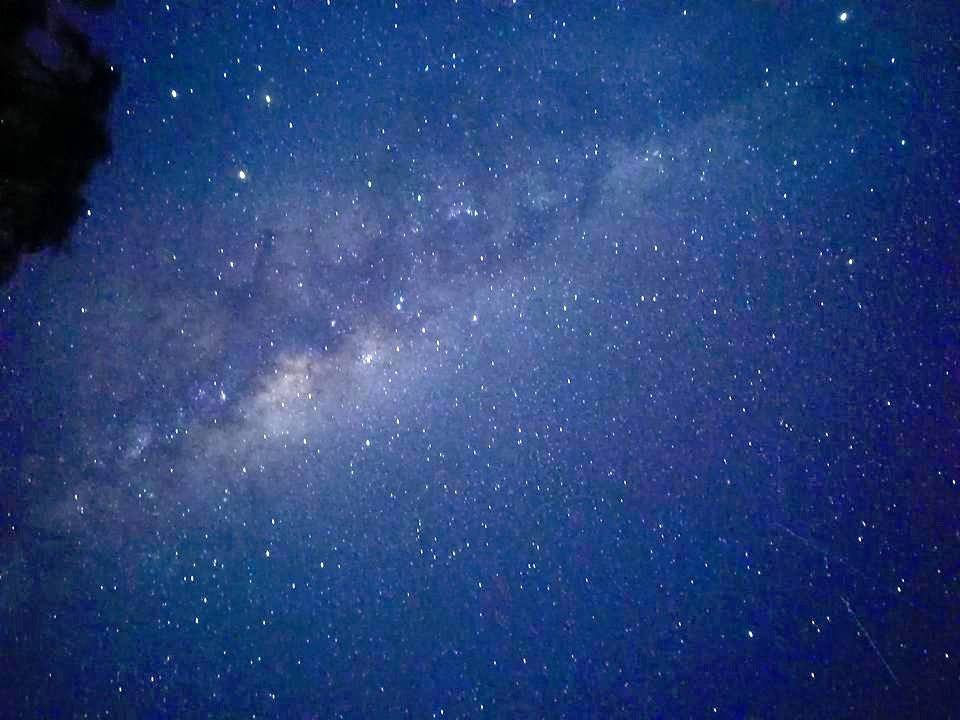
\includegraphics[width=0.95\textwidth]{aus-sky-5.jpg}
}

\frame{
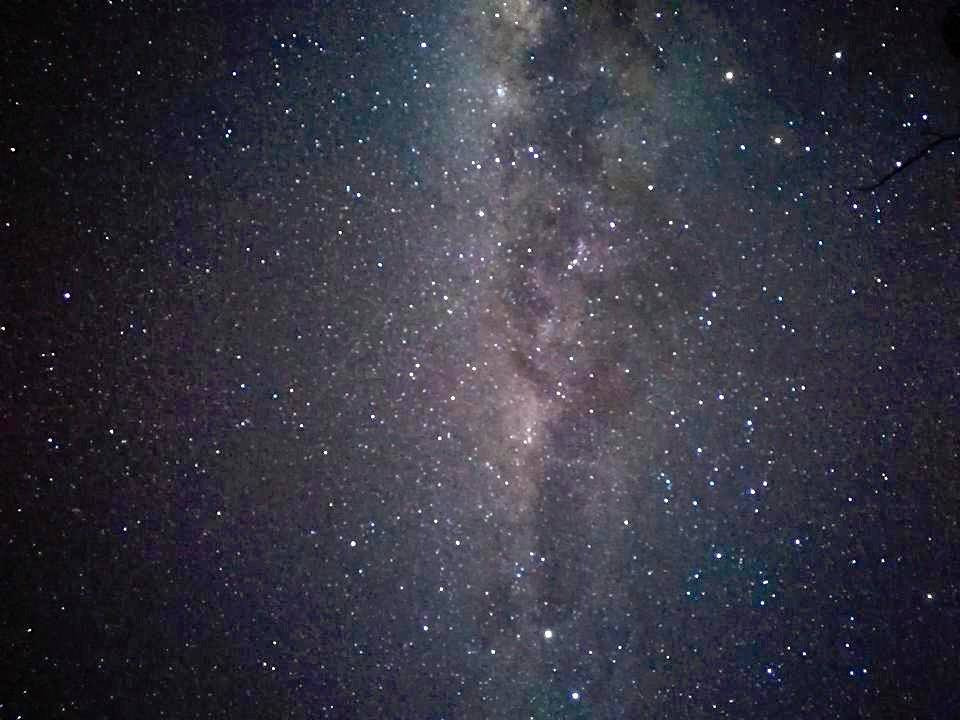
\includegraphics[width=0.95\textwidth]{aus-sky-4.jpg}
}

\frame{
\BC \Large
A friend of one of your classmates took these recently in Australia.

\bigskip
\bigskip

He thinks they were taken with a cellphone camera. This seems plausible!

\bigskip
\bigskip
\pause

... you can capture light from thousands of light-years away with an imager a centimeter across!
\EC
}

\frame{
\BC
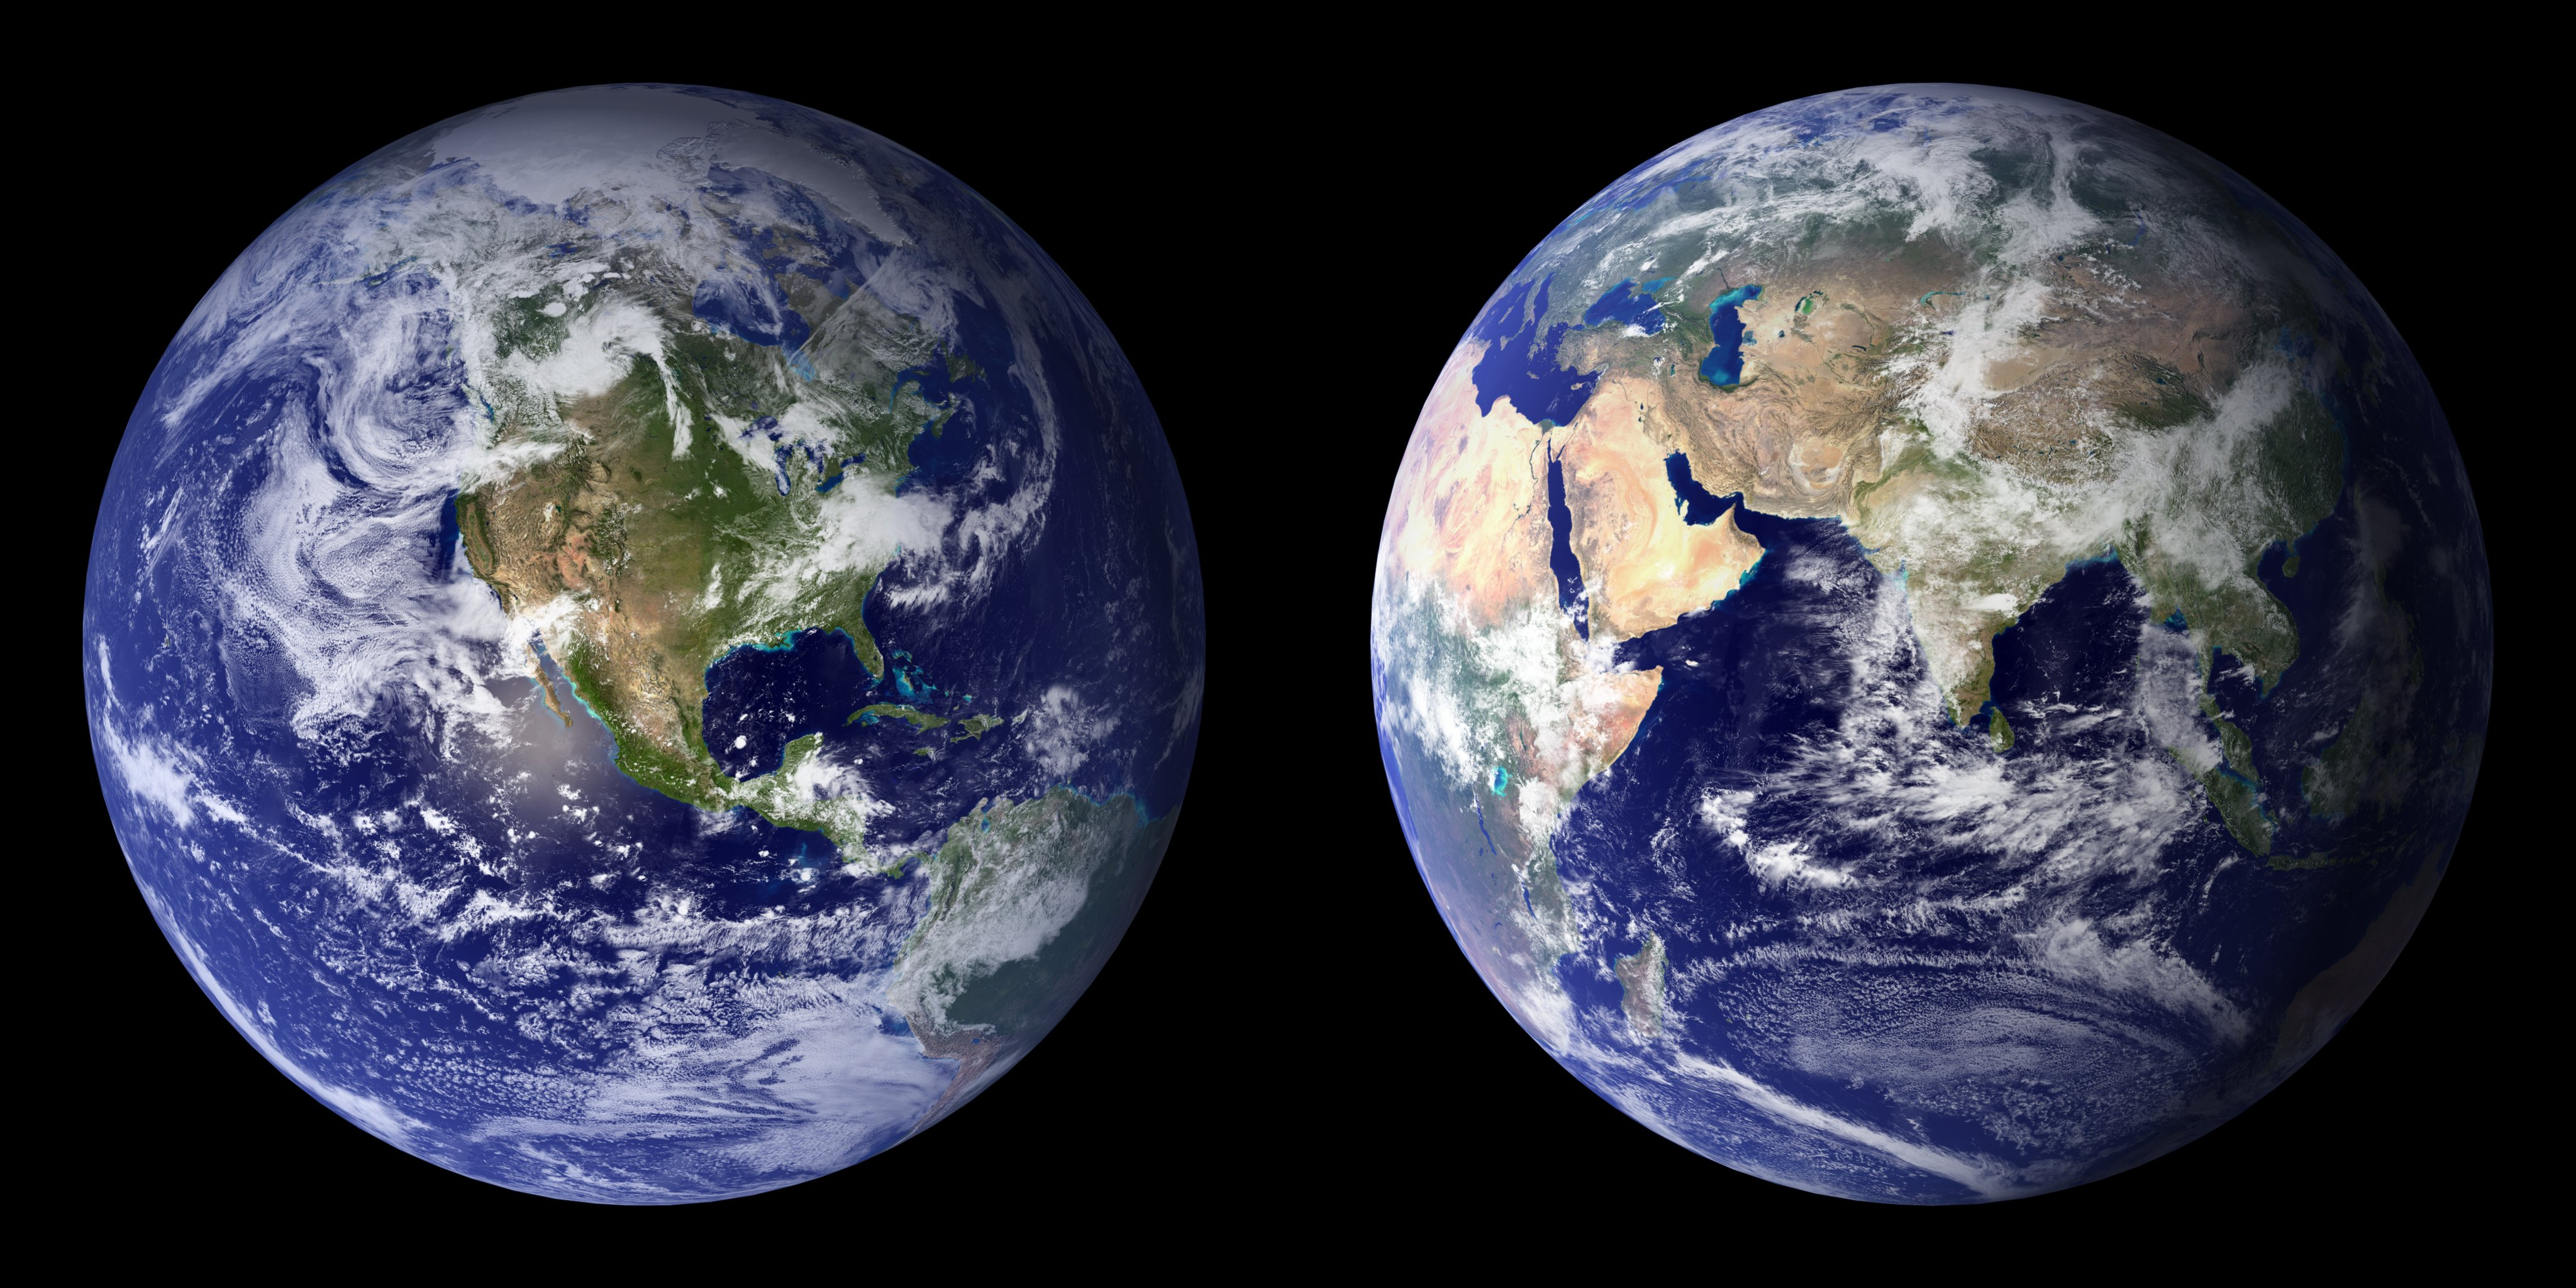
\includegraphics[width=\textwidth]{blue-marble.jpg}

\bigskip
\Large
What kind of world is this? What {\it can't} you see?
\EC
}

\frame{
\BC
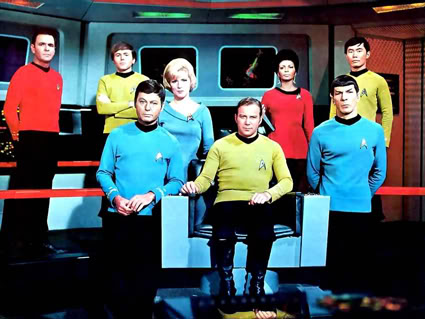
\includegraphics[width=0.8\textwidth]{star-trek-cast.jpg}

\bigskip
\Large
Cast of {\it Star Trek}, 1968
\EC
}


\frame{\frametitle{\textbf{Some announcements}}
\Large
\BI
\item{Homework 1 postponed until next Thursday (you'll need some of Tuesday's material for it)}
\item{Labs start next week}
\EI
}


\frame{\frametitle{\textbf{Some announcements}}
\Large
I called the bookstore Tuesday.

\BI
\item{They got an order in that morning}
\item{All of the books went to people who preordered}
\item{More should be in today}
\item{Make an online preorder reservation to get yours first}
\EI
}

\frame{\frametitle{\textbf{Help sessions}}
\Large
Lots of people came by Tuesday asking some very good questions.

\bigskip
\bigskip
\bigskip

This is the absolute very best thing you can do to study for my class.

\bigskip
\bigskip

Come by the Clinic, Physics Building 112, and ask questions!
}


\frame{\frametitle{\textbf{This week we will...}}
\Large
Today: consequences of the Earth's {\bf revolution}:
\BI
\item{How is the Sun different from the other stars?}
\item{What's this zodiac business?}
\item{What does it mean for the Sun to be ``in Aries''?}
\pause
\item{We will see how this is only complicated because of {\bf how we keep time}}
\EI
}

\frame{\frametitle{\textbf{Which is true about the Sun?}}
\large
\color{A}A: The celestial sphere model predicts its motion exactly\\
\bigskip
\color{B}B: The celestial sphere model predicts its daily motion, but isn't accurate for longer times \\
\bigskip
\color{C}C: The celestial sphere model is completely wrong for the Sun
\bigskip
}

\frame{
\Large

Why is the celestial sphere model a bit wrong for the Sun?

\bigskip
\bigskip
\bigskip
\bigskip

\color{A}A: The Sun is close enough that the Earth's movement matters, unlike for other stars \\
\bigskip
\color{B}B: The Sun lies on a different celestial sphere than the stars, which turns at a different rate \\
\bigskip
\color{C}C: Angels push the Sun around on the celestial sphere, so it moves \\
\bigskip
\color{D}D: The Sun is close enough that we notice its movement, unlike the other stars
}

\frame{\frametitle{\textbf{A demonstration}}
\Large
Let's use {\it Stellarium} to revisit the same time every night -- say, midnight.

\pause\bigskip\bigskip

... What's wrong?

\pause\bigskip\bigskip

... isn't the celestial sphere supposed to rotate once per day?

... Why are the stars moving?

... What's wrong?

}


\frame{\frametitle{\textbf{A demonstration}}
\Large
Now let's look at the sky during the {\it daytime}, pretending the atmosphere is gone.

\bigskip
\bigskip
\bigskip

\pause

Which moves more, the sun or the stars?

\bigskip
\bigskip
\bigskip
\pause

\BI
\item{The Sun just moves up and down a little bit, and the stars spin!}
\item{... why is this?}
\EI
}

\frame{
\Huge
\BC Let's animate this and try to understand. \EC
}

\frame{
\Huge
\BC Work through the {\it Lecture Tutorials}, pp. 7-9. \EC

\bigskip
\BC \large We will talk about something else after this.
\EC
}



\frame{
\Large

\begin{columns}
\column{0.5\textwidth}
Which image shows the position of the Earth {\it \bf exactly} one day later?

\bigskip
\bigskip
\bigskip

\color{A}A: Noon \\
\color{B}B: Midnight \\
\color{C}C: Sunrise \\
\color{D}D: Sunset 
\column{0.5\textwidth}
\BC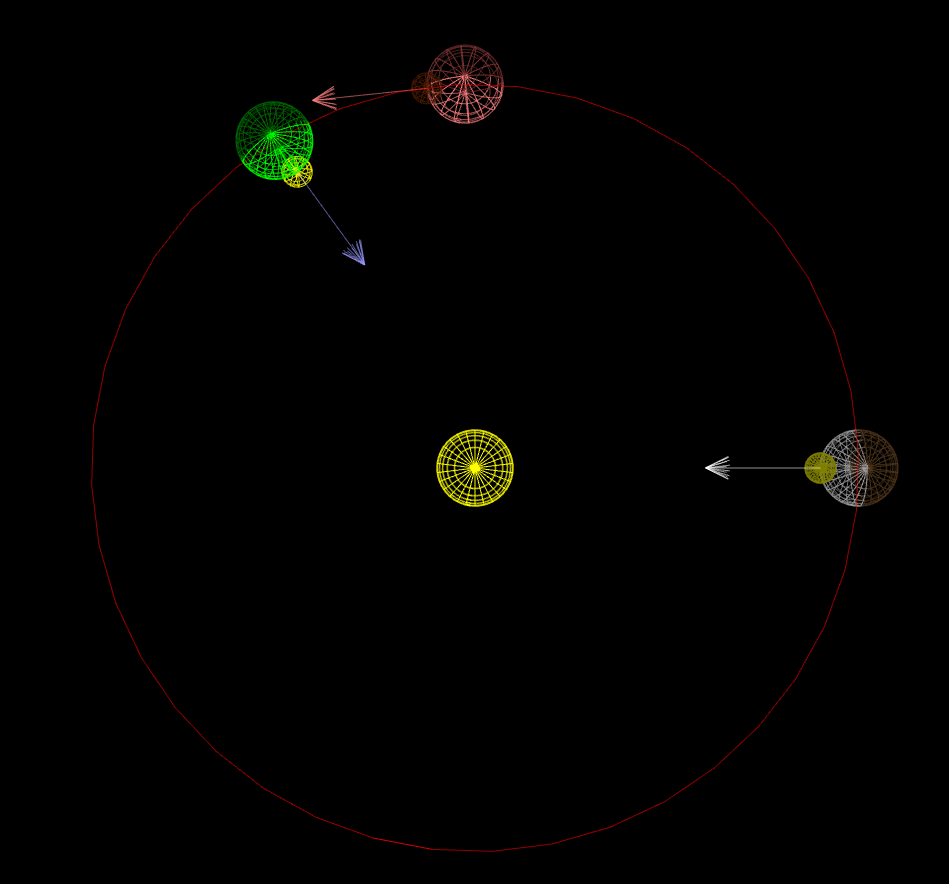
\includegraphics[width=0.9\textwidth]{day-question-1.png}\EC
\end{columns}

}

\frame{
\Large
\begin{columns}
\column{0.5\textwidth}
Which image shows the position of the Earth {\it \bf exactly} one day later?
\column{0.5\textwidth}
\BC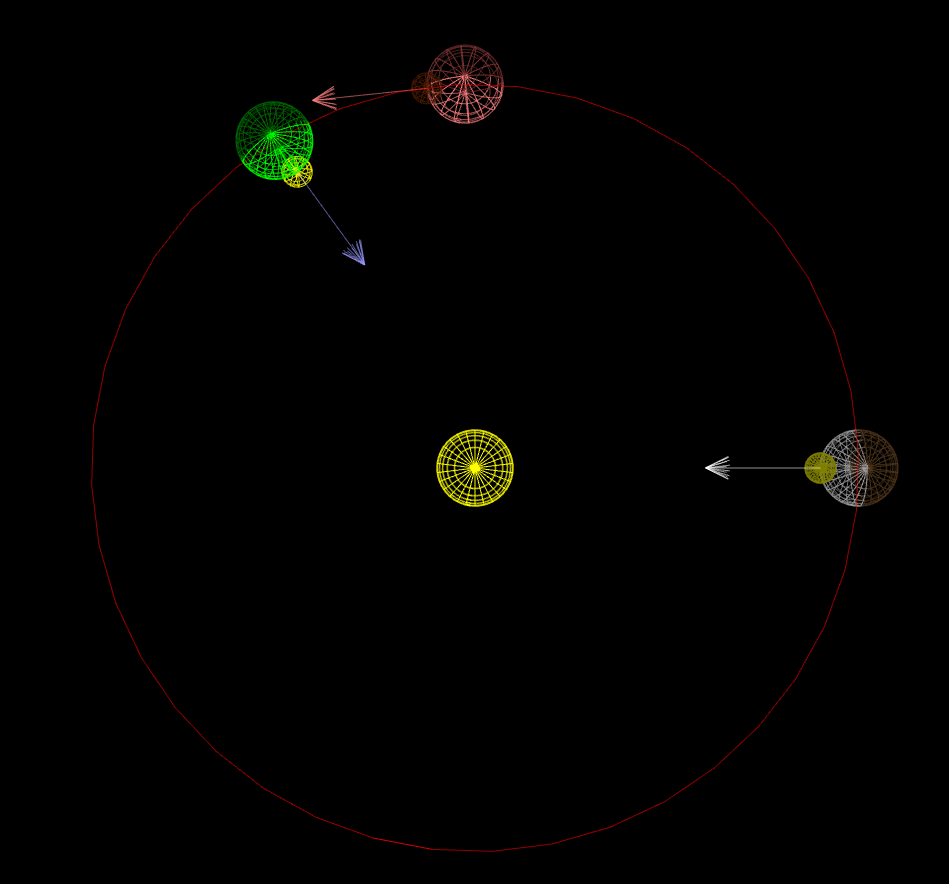
\includegraphics[width=0.9\textwidth]{day-question-1.png}\EC
\end{columns}

\bigskip
\bigskip

\color{A}A: The red one \\
\color{B}B: The green one \\
\pause
\color{C}C: Depends on what you mean by ``a day'' \\
\pause
\color{D}D: The Earth moves? BURN THE HERETIC!

}


\frame{
\Large
There are {\it two kinds} of day!

\BI
\item{Solar day: judged by the position of the Sun}
\item{Sidereal day (sih-dee-ree-al): judged only by the rotation of the Earth with respect to the stars}
\EI
}

\frame{

\BC\Huge Work through the {\it Lecture Tutorials}, pp. 11-12.

\bigskip

\large
We will talk about something else after this.
\EC
}

\frame{\frametitle{\textbf{Two kinds of day!}}
\Large

\BC Demo in {\it Stellarium:} \EC

\bigskip
\bigskip
\begin{columns}
\column{0.5\textwidth}
\Large
In one solar day...
\column{0.5\textwidth}
\Large
In one sidereal day...
\end{columns}
\begin{columns}
\column{0.5\textwidth}
\BI
\large
\item{The stars move a lot}
\item{...since the Earth isn't pointed in the same direction}
\item{The Sun moves higher or lower in the sky a little bit}
\item{Exactly 24h}
\EI

\column{0.5\textwidth}
\BI
\large
\item{The stars don't move at all}
\item{... since the Earth is pointed in the same direction}
\item{The Sun moves a lot, since the Earth has moved}
\item{A little bit less than 24h}
\EI
\end{columns}
}

\frame{\frametitle{Lecture tutorials, again}
\Huge
\BC
Complete pp. 12-16.
\EC

\large
\bigskip
If you don't have time to finish, that's okay. Finishing this is great practice at home, though!

\bigskip
\bigskip
\bigskip
\bigskip
\pause
\large
\BC Live long and prosper!\EC
}


\end{document}
